\documentclass[8pt,aspectratio=169]{beamer}
\usetheme{Madrid}
\usecolortheme{default}

\usepackage{amsmath,amssymb}
\usepackage{graphicx}
\usepackage{booktabs}
\usepackage{tikz}
\usetikzlibrary{arrows.meta,positioning}

\title{Private Credit Case Study}
\subtitle{CLO Portfolio Analysis with Deep Generative Models}
\author{Digital AI Finance}
\date{2026}

\setbeamertemplate{navigation symbols}{}
\setbeamertemplate{footline}[frame number]

\begin{document}

\begin{frame}
\titlepage
\end{frame}

\begin{frame}{Outline}
\tableofcontents
\end{frame}

%------------------------------------------------------------
\section{Portfolio Overview}
%------------------------------------------------------------

\begin{frame}{Case Study: Middle Market CLO}
\textbf{Portfolio Characteristics}:
\begin{itemize}
    \item Total Size: \$500 million
    \item Number of Loans: 500
    \item Weighted Average Spread: L+450 bps
    \item Weighted Average Life: 4.2 years
\end{itemize}

\vspace{0.5em}
\textbf{Asset Mix}:
\begin{table}
\centering
\begin{tabular}{lcc}
\toprule
Asset Class & Weight & Avg. PD \\
\midrule
Corporate First Lien & 60\% & 2.0\% \\
Corporate Second Lien & 15\% & 3.5\% \\
Consumer ABS & 15\% & 4.0\% \\
CRE Bridge & 10\% & 2.5\% \\
\bottomrule
\end{tabular}
\end{table}
\end{frame}

\begin{frame}{Capital Structure}
\begin{table}
\centering
\begin{tabular}{lccccc}
\toprule
Tranche & Rating & Size (\$M) & \% & Att. & Det. \\
\midrule
Class A & AAA & 350 & 70\% & 30\% & 100\% \\
Class B & AA & 40 & 8\% & 22\% & 30\% \\
Class C & A & 30 & 6\% & 16\% & 22\% \\
Class D & BBB & 30 & 6\% & 10\% & 16\% \\
Class E & BB & 25 & 5\% & 5\% & 10\% \\
Equity & NR & 25 & 5\% & 0\% & 5\% \\
\midrule
\textbf{Total} & & \textbf{500} & \textbf{100\%} & & \\
\bottomrule
\end{tabular}
\end{table}

\vspace{0.5em}
\textbf{Key metrics}:
\begin{itemize}
    \item AAA Subordination: 30\%
    \item Equity cushion: 5\%
    \item Overcollateralization: 103\%
\end{itemize}
\end{frame}

%------------------------------------------------------------
\section{Data Preparation}
%------------------------------------------------------------

\begin{frame}{Loan Tape Structure}
\textbf{Required fields per loan}:
\begin{table}
\centering
\footnotesize
\begin{tabular}{ll}
\toprule
Field & Description \\
\midrule
\texttt{loan\_id} & Unique identifier \\
\texttt{origination\_date} & Loan start date \\
\texttt{original\_balance} & Initial principal \\
\texttt{current\_balance} & Outstanding principal \\
\texttt{interest\_rate} & Coupon rate \\
\texttt{maturity\_date} & Scheduled maturity \\
\texttt{asset\_class} & Corporate, Consumer, RE, etc. \\
\texttt{credit\_rating} & Internal rating (1-10) \\
\texttt{current\_state} & Performing, 30DPD, etc. \\
\texttt{collateral\_type} & First lien, Second lien, etc. \\
\bottomrule
\end{tabular}
\end{table}

\vspace{0.5em}
\textbf{Panel data}: Monthly observations with state and payment info.
\end{frame}

\begin{frame}[fragile]{Data Loading}
\begin{verbatim}
from privatecredit.data import LoanTapeGenerator

# Load historical loan tape
generator = LoanTapeGenerator(
    n_loans=500,
    start_date='2020-01-01',
    seed=42
)

loans, panel = generator.generate(
    asset_mix={'corporate': 0.75, 'consumer': 0.15, 'cre': 0.10},
    target_pd=0.025,
    target_lgd=0.40
)

print(f"Loans: {len(loans)}")
print(f"Panel observations: {len(panel)}")
\end{verbatim}

\vspace{0.5em}
\textbf{Output}: 500 loans $\times$ 60 months = 30,000 observations
\end{frame}

\begin{frame}{Macro Data Preparation}
\textbf{Historical macro variables} (60 months):
\begin{itemize}
    \item GDP Growth (YoY)
    \item Unemployment Rate
    \item CPI Inflation
    \item Fed Funds Rate
    \item 10Y Treasury Yield
    \item IG Credit Spread
    \item HY Credit Spread
    \item Commercial Property Index
    \item Equity Returns
\end{itemize}

\vspace{0.5em}
\textbf{Sources}: FRED, Bloomberg, proprietary indices

\vspace{0.5em}
\textbf{Processing}:
\begin{itemize}
    \item Standardize to monthly frequency
    \item Handle missing values (forward fill)
    \item Normalize for model input
\end{itemize}
\end{frame}

%------------------------------------------------------------
\section{Model Training}
%------------------------------------------------------------

\begin{frame}[fragile]{Training Macro VAE}
\begin{verbatim}
from privatecredit.models import MacroVAE, MacroVAEConfig

config = MacroVAEConfig(
    n_macro_vars=9,
    seq_length=60,
    latent_dim=32,
    hidden_dim=128,
    n_scenarios=4
)

vae = MacroVAE(config)
vae.fit(
    train_data=macro_train,
    epochs=100,
    batch_size=32,
    lr=1e-3,
    beta_schedule='cyclical'
)
\end{verbatim}

\textbf{Training time}: ~15 minutes on GPU
\end{frame}

\begin{frame}{Training Results: Macro VAE}
\textbf{Loss convergence}:
\begin{itemize}
    \item Final ELBO: -125.3
    \item Reconstruction MSE: 0.023
    \item KL Divergence: 12.4
\end{itemize}

\vspace{0.5em}
\textbf{Quality metrics}:
\begin{table}
\centering
\begin{tabular}{lcc}
\toprule
Metric & Target & Achieved \\
\midrule
GDP Mean & 2.5\% & 2.48\% \\
GDP Std & 1.5\% & 1.52\% \\
GDP-Unemp Corr & -0.65 & -0.63 \\
Autocorrelation & 0.90 & 0.88 \\
\bottomrule
\end{tabular}
\end{table}

\vspace{0.5em}
Generated scenarios match historical distributions.
\end{frame}

\begin{frame}[fragile]{Training Transition Transformer}
\begin{verbatim}
from privatecredit.models import TransitionTransformer

transformer = TransitionTransformer(
    n_states=7,
    n_macro_vars=9,
    hidden_dim=128,
    n_heads=4,
    n_layers=4
)

transformer.fit(
    macro_paths=macro_train,
    transition_targets=cohort_transitions,
    epochs=50
)
\end{verbatim}

\textbf{Training time}: ~10 minutes on GPU
\end{frame}

%------------------------------------------------------------
\section{Scenario Analysis}
%------------------------------------------------------------

\begin{frame}{Scenario Generation}
\textbf{Four scenarios generated}:

\begin{table}
\centering
\footnotesize
\begin{tabular}{lcccc}
\toprule
Variable & Baseline & Adverse & Severe & Stagflation \\
\midrule
GDP Growth & 2.5\% & 0.5\% & -2.0\% & 0.5\% \\
Unemployment & 4.0\% & 6.5\% & 10.0\% & 7.0\% \\
Inflation & 2.0\% & 1.5\% & 1.0\% & 5.0\% \\
HY Spread & 400 bps & 650 bps & 1000 bps & 700 bps \\
\bottomrule
\end{tabular}
\end{table}

\vspace{0.5em}
\textbf{Scenario probability weights}:
\begin{itemize}
    \item Baseline: 60\%
    \item Adverse: 25\%
    \item Severely Adverse: 10\%
    \item Stagflation: 5\%
\end{itemize}
\end{frame}

\begin{frame}{Default Rate Projections}
\textbf{Cumulative default rates by scenario}:

\begin{table}
\centering
\begin{tabular}{lcccc}
\toprule
Month & Baseline & Adverse & Severe & Stagflation \\
\midrule
12 & 1.2\% & 2.5\% & 4.0\% & 3.0\% \\
24 & 2.8\% & 5.5\% & 9.0\% & 6.5\% \\
36 & 4.5\% & 8.5\% & 14.0\% & 10.0\% \\
48 & 6.2\% & 11.0\% & 18.5\% & 13.0\% \\
60 & 8.0\% & 13.5\% & 22.0\% & 15.5\% \\
\bottomrule
\end{tabular}
\end{table}

\vspace{0.5em}
\textbf{Key insight}: Severely adverse scenario implies 22\% cumulative defaults over 5 years.
\end{frame}

\begin{frame}{PD Multipliers by Scenario}
\textbf{Monthly PD stress multipliers}:

\begin{tikzpicture}
\begin{axis}[
    width=0.9\textwidth,
    height=0.6\textheight,
    xlabel={Month},
    ylabel={PD Multiplier},
    legend pos=north west,
    grid=major,
    ymin=0.5,
    ymax=5
]
\addplot[blue, thick] coordinates {(0,1) (12,1) (24,1) (36,1) (48,1) (60,1)};
\addlegendentry{Baseline}
\addplot[orange, thick] coordinates {(0,1) (12,1.8) (24,2.2) (36,2.0) (48,1.8) (60,1.5)};
\addlegendentry{Adverse}
\addplot[red, thick] coordinates {(0,1) (12,2.5) (24,4.0) (36,3.5) (48,3.0) (60,2.5)};
\addlegendentry{Severe}
\addplot[purple, thick] coordinates {(0,1) (12,2.0) (24,2.8) (36,2.5) (48,2.2) (60,2.0)};
\addlegendentry{Stagflation}
\end{axis}
\end{tikzpicture}
\end{frame}

%------------------------------------------------------------
\section{Monte Carlo Simulation}
%------------------------------------------------------------

\begin{frame}{Simulation Setup}
\textbf{Monte Carlo parameters}:
\begin{itemize}
    \item Number of simulations: 10,000
    \item Time horizon: 60 months
    \item Asset correlation: 15\%
    \item LGD: 40\% (beta distributed)
\end{itemize}

\vspace{0.5em}
\textbf{Model}: Vasicek single-factor
\begin{equation}
A_i = \sqrt{\rho} Z + \sqrt{1-\rho} \epsilon_i
\end{equation}

\vspace{0.5em}
\textbf{Default condition}:
\begin{equation}
D_i = \mathbf{1}_{A_i < \Phi^{-1}(\text{PD}_i)}
\end{equation}
\end{frame}

\begin{frame}{Loss Distribution Results}
\textbf{Portfolio loss statistics}:

\begin{table}
\centering
\begin{tabular}{lcc}
\toprule
Metric & Value & \% of Portfolio \\
\midrule
Expected Loss & \$6.0M & 1.2\% \\
Standard Deviation & \$4.5M & 0.9\% \\
VaR (95\%) & \$12.5M & 2.5\% \\
VaR (99\%) & \$18.2M & 3.6\% \\
CVaR (99\%) & \$22.8M & 4.6\% \\
Maximum Loss & \$42.0M & 8.4\% \\
\bottomrule
\end{tabular}
\end{table}

\vspace{0.5em}
\textbf{Key finding}: 99\% VaR (3.6\%) is well below AAA subordination (30\%).
\end{frame}

\begin{frame}{Tranche Loss Analysis}
\textbf{Expected loss by tranche}:

\begin{table}
\centering
\begin{tabular}{lccc}
\toprule
Tranche & Size & Exp. Loss & Loss Rate \\
\midrule
AAA & \$350M & \$0.0M & 0.00\% \\
AA & \$40M & \$0.0M & 0.00\% \\
A & \$30M & \$0.0M & 0.01\% \\
BBB & \$30M & \$0.1M & 0.33\% \\
BB & \$25M & \$0.8M & 3.20\% \\
Equity & \$25M & \$5.1M & 20.40\% \\
\midrule
\textbf{Total} & \$500M & \$6.0M & 1.20\% \\
\bottomrule
\end{tabular}
\end{table}

\vspace{0.5em}
\textbf{Observation}: Equity absorbs 85\% of expected losses.
\end{frame}

\begin{frame}{Stress Scenario Impact}
\textbf{VaR 99\% by scenario}:

\begin{table}
\centering
\begin{tabular}{lcc}
\toprule
Scenario & VaR 99\% & First Loss Tranche \\
\midrule
Baseline & \$18.2M (3.6\%) & BB (partial) \\
Adverse & \$32.0M (6.4\%) & BBB (partial) \\
Severely Adverse & \$55.0M (11.0\%) & A (partial) \\
Stagflation & \$40.0M (8.0\%) & BBB \\
\bottomrule
\end{tabular}
\end{table}

\vspace{0.5em}
\textbf{Stress test conclusion}:
\begin{itemize}
    \item AAA remains protected even in severely adverse scenario
    \item AA faces risk only in extreme tail ($>$99.9\%)
    \item Equity fully wiped in adverse scenario
\end{itemize}
\end{frame}

%------------------------------------------------------------
\section{Risk Metrics}
%------------------------------------------------------------

\begin{frame}{Coverage Ratios}
\textbf{Interest Coverage (IC)}:
\begin{equation}
\text{IC}_k = \frac{\text{Interest Collections} - \text{Fees}}{\sum_{j \leq k} \text{Tranche}_j \times \text{Rate}_j}
\end{equation}

\vspace{0.5em}
\begin{table}
\centering
\begin{tabular}{lccc}
\toprule
Tranche & IC Baseline & IC Adverse & Trigger \\
\midrule
AAA & 1.85 & 1.52 & 1.20 \\
AA & 1.65 & 1.35 & 1.15 \\
A & 1.48 & 1.21 & 1.10 \\
BBB & 1.32 & 1.08 & 1.05 \\
BB & 1.18 & 0.97 & 1.00 \\
\bottomrule
\end{tabular}
\end{table}

\vspace{0.5em}
\textbf{Warning}: BB IC falls below trigger in adverse scenario.
\end{frame}

\begin{frame}{Overcollateralization}
\textbf{OC Ratios}:
\begin{equation}
\text{OC}_k = \frac{\text{Portfolio NAV}}{\sum_{j \leq k} \text{Tranche}_j \text{ (outstanding)}}
\end{equation}

\vspace{0.5em}
\begin{table}
\centering
\begin{tabular}{lccc}
\toprule
Tranche & OC Initial & OC Stressed & Trigger \\
\midrule
AAA & 1.43 & 1.31 & 1.20 \\
AA & 1.28 & 1.17 & 1.12 \\
A & 1.19 & 1.09 & 1.08 \\
BBB & 1.11 & 1.02 & 1.04 \\
\bottomrule
\end{tabular}
\end{table}

\vspace{0.5em}
\textbf{Action}: BBB OC breach triggers cash flow diversion.
\end{frame}

%------------------------------------------------------------
\section{Results Interpretation}
%------------------------------------------------------------

\begin{frame}{Rating Agency View}
\textbf{Implied ratings from loss analysis}:

\begin{table}
\centering
\begin{tabular}{lccc}
\toprule
Tranche & Target & Implied & Cushion \\
\midrule
AAA & 0.01\% & 0.00\% & +100\% \\
AA & 0.10\% & 0.02\% & +80\% \\
A & 0.50\% & 0.15\% & +70\% \\
BBB & 1.50\% & 0.85\% & +43\% \\
BB & 5.00\% & 3.20\% & +36\% \\
\bottomrule
\end{tabular}
\end{table}

\vspace{0.5em}
\textbf{Assessment}: All tranches meet rating targets with comfortable cushion.
\end{frame}

\begin{frame}{Sensitivity Analysis}
\textbf{Impact of key parameters}:

\begin{table}
\centering
\footnotesize
\begin{tabular}{lccc}
\toprule
Parameter Change & EL Impact & VaR 99\% Impact & First Affected \\
\midrule
PD +50\% & +52\% & +48\% & BB \\
LGD +10pp & +25\% & +28\% & Equity \\
Correlation +5pp & +8\% & +35\% & BBB \\
Concentration +20\% & +5\% & +22\% & BB \\
\bottomrule
\end{tabular}
\end{table}

\vspace{0.5em}
\textbf{Key driver}: Correlation has outsized impact on tail risk.
\end{frame}

\begin{frame}{Management Actions}
\textbf{Recommendations based on analysis}:

\begin{enumerate}
    \item \textbf{Reduce concentration}
    \begin{itemize}
        \item Top 10 obligors: 15\% $\rightarrow$ 10\%
        \item Reduces VaR by ~12\%
    \end{itemize}

    \item \textbf{Increase subordination}
    \begin{itemize}
        \item BB attachment: 5\% $\rightarrow$ 7\%
        \item Improves BB rating cushion
    \end{itemize}

    \item \textbf{Tighten OC triggers}
    \begin{itemize}
        \item Earlier cash flow diversion
        \item Protects senior tranches
    \end{itemize}

    \item \textbf{Stress test monitoring}
    \begin{itemize}
        \item Monthly scenario updates
        \item Early warning system
    \end{itemize}
\end{enumerate}
\end{frame}

%------------------------------------------------------------
\section{Summary}
%------------------------------------------------------------

\begin{frame}{Key Findings}
\begin{enumerate}
    \item \textbf{Portfolio Quality}
    \begin{itemize}
        \item Expected loss: 1.2\% (acceptable)
        \item Senior tranches well protected
    \end{itemize}

    \item \textbf{Stress Resilience}
    \begin{itemize}
        \item AAA survives severely adverse scenario
        \item Equity absorbs first 5\% losses
    \end{itemize}

    \item \textbf{Risk Drivers}
    \begin{itemize}
        \item Correlation most impacts tail risk
        \item Concentration adds 22\% to VaR
    \end{itemize}

    \item \textbf{Model Value}
    \begin{itemize}
        \item Scenario-specific insights
        \item Granular loan-level analysis
        \item Differentiable end-to-end
    \end{itemize}
\end{enumerate}
\end{frame}

\begin{frame}{Next Steps}
\textbf{Deployment}:
\begin{itemize}
    \item Production API for real-time risk metrics
    \item Automated monthly scenario updates
    \item Integration with reporting systems
\end{itemize}

\vspace{0.5em}
\textbf{Enhancements}:
\begin{itemize}
    \item Add prepayment model refinement
    \item Incorporate recovery timing
    \item Extend to multi-asset CLOs
\end{itemize}

\vspace{0.5em}
\textbf{Documentation}:
\begin{itemize}
    \item Full methodology paper
    \item Interactive demos
    \item Training materials
\end{itemize}
\end{frame}

\begin{frame}{}
\begin{center}
\Huge Thank You

\vspace{1em}
\Large Questions?

\vspace{2em}
\normalsize
\url{https://digital-ai-finance.github.io/private-credit/}
\end{center}
\end{frame}

\end{document}
